\begin{frame}
    \centering
    \begin{figure}[H]
        
\includegraphics[keepaspectratio, width=0.7\paperwidth, height=\paperheight]{LeeLogo}
    \end{figure}
    Informatik: Data Science und Sicherheit\\
     \textbf{Netzwerke} \emoji{computer} \emoji{globe-with-meridians}
\end{frame}

\begin{frame}[fragile]{Was sind Netzwerke?}
    \begin{itemize}
    \item Graphen:
                \begin{figure}[H]
                \centering
                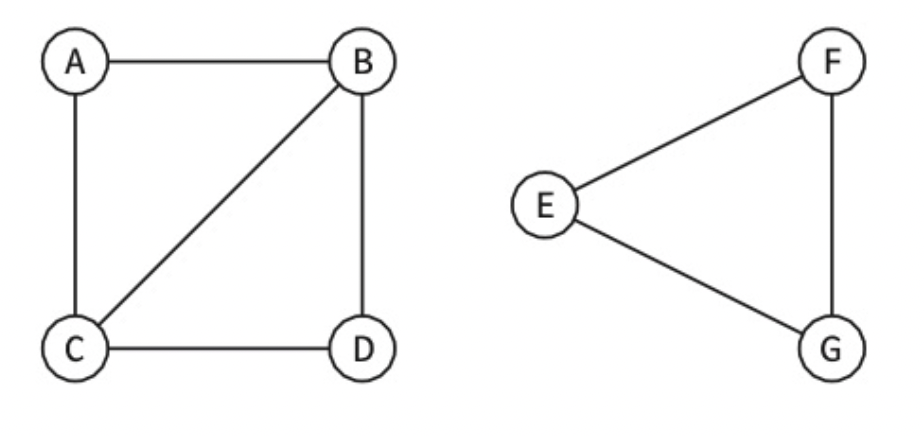
\includegraphics[keepaspectratio, width=0.35 \paperwidth]{GrundlagenInfo/02_Graphen/Figures/4-graph-zusammenhaengend.png}
            \end{figure}    
    
	    \item Im Alltag: 
	    \begin{itemize}
		    \item Post
		    \item Soziale Netzwerke
		    \item SBB, Zugverbindungen
		    \item Aliexpress, Uber, ...
		    \item \textbf{Das Internet}
	    \end{itemize}
    \end{itemize}
\end{frame}

\begin{frame}[fragile]{Was sind Netzwerke?}
    \begin{itemize}
    \item Graphen:
                \begin{figure}[H]
                \centering
                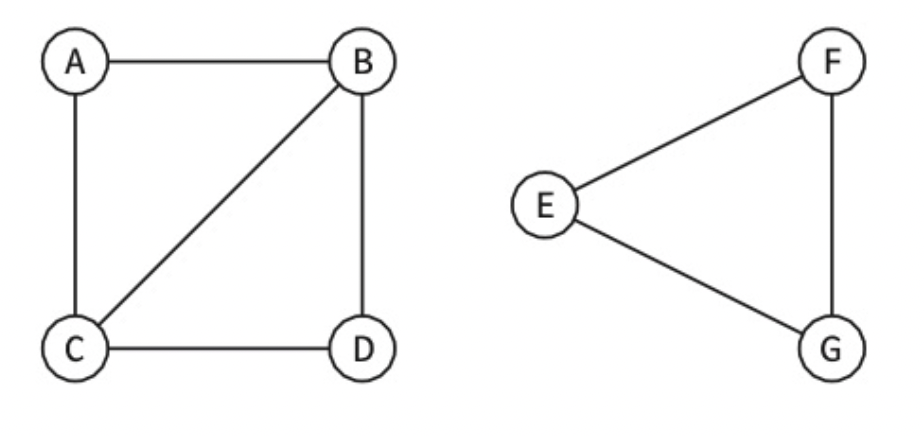
\includegraphics[keepaspectratio, width=0.35 \paperwidth]{GrundlagenInfo/02_Graphen/Figures/4-graph-zusammenhaengend.png}
            \end{figure}    
    
	    \item Im Alltag: 
	    \begin{itemize}
		    \item Post
		    \item Soziale Netzwerke
		    \item SBB, Zugverbindungen
		    \item Aliexpress, Uber, ...
		    \item \textbf{Das Internet}
	    \end{itemize}
    \end{itemize}
\end{frame}

\begin{frame}[fragile]{Internet: Analogie}{Wie war es früher?}
\begin{figure}[H]
\centering
\begin{tikzpicture}[
    auto,
    block/.style={
	    minimum width=3cm,
	    node distance=1.5cm,
        rectangle, 
        fill=RoyalBlue!50, 
        align=center, 
        rounded corners
    }
]


% Define the nodes with FontAwesome icons
\node[block] (chefs) {\faFemale\ Chef};
\node[block, below=of chefs] (secretariat) {\faPhone\ Sekretariat};
\node[block, below=of secretariat] (postman) {\faMale\ Post};


% Define the nodes with FontAwesome icons

\node[block, right=of postman] (postman2) {\faMale\ Post};
\node[block, above=of postman2] (secretariat2) {\faPhone\ Sekretariat};
\node[block, above=of secretariat2] (chefs2) {\faMale\ Chef};


% Draw the dashed arrows
\draw[<->, dashed, RoyalBlue!50, thick] (chefs) -- (chefs2);
\draw[<->, dashed, RoyalBlue!50, thick] (secretariat) -- (secretariat2);
\draw[<->, dashed, RoyalBlue!50, thick] (postman) -- (postman2);

\draw[->, line width=1mm,ForestGreen!50] (chefs) -- node[left]{\faComments} (secretariat) ;
\draw[->, line width=1mm,ForestGreen!50] (secretariat) -- node[left]{\faEnvelope} (postman) ;
\draw[->, line width=1mm,ForestGreen!50, bend right] (postman.south) to node[midway,below]{\faBicycle\ \faMotorcycle\ \faCar\ \faShip\ \faPlane} (postman2.south) ;
\draw[->, line width=1mm,ForestGreen!50] (postman2) -- node[right]{\faEnvelope} (secretariat2) ;
\draw[->, line width=1mm,ForestGreen!50] (secretariat2) -- node[right]{\faComments} (chefs2) ;

% fit rectangles around regions
\node[fit=(chefs) (postman), inner sep=8pt, red, dotted, draw, line width=1pt,rounded corners](region1) {};
\node[fit=(chefs2) (postman2), inner sep=8pt, red, dotted, draw, line width=1pt,rounded corners](region2) {};
% annotate both rectangles
\node[above=5pt of region1.north, anchor=center, align=center]{\textcolor{red}{Firma 1, Europa}};
\node[above=5pt of region2.north, anchor=center, align=center]{\textcolor{red}{Firma 2, Asien}};

\end{tikzpicture}
\end{figure}
\end{frame}

\begin{frame}[fragile]{...}
\begin{figure}[H]
...
\end{figure}
\end{frame}